%----------------------------------------------------------------------------------------
% DOCUMENT CONFIGURATION
%----------------------------------------------------------------------------------------
\documentclass[10pt,english,french]{article}

%----------------------------------------------------------------------------------------
% ENCODING
%----------------------------------------------------------------------------------------
\usepackage[T1]{fontenc}
\usepackage[utf8]{inputenc}
\usepackage[USenglish, french]{isodate}
\usepackage{fancyhdr}
\usepackage[numbers]{natbib}

%----------------------------------------------------------------------------------------
% LOGIC
%----------------------------------------------------------------------------------------
\usepackage{xstring, xifthen}
\usepackage{enumitem}
\usepackage[english, french]{babel}
\usepackage{blindtext}
\usepackage{pdfpages}
\usepackage{changepage}
\usepackage{etoolbox}
\usepackage{tabularx}

%----------------------------------------------------------------------------------------
% FONT SETTINGS
%----------------------------------------------------------------------------------------
% -------> Roboto
% \usepackage[sfdefault]{roboto}
% \renewcommand*\familydefault{\sfdefault}
% \renewcommand{\familydefault}{\sfdefault}
% \usepackage{moresize}
% -------> TeX Gyre Heros
% \usepackage{tgheros}
% \renewcommand{\familydefault}{\sfdefault}
% -------> Source Sans Pro
% \usepackage[default]{sourcesanspro}
% \renewcommand*\familydefault{\sfdefault}
% -------> To use LaTeX default font do not include any font package

%----------------------------------------------------------------------------------------
% ICONS / EMOJIS
%----------------------------------------------------------------------------------------
\usepackage{xparse}
\usepackage{twemojis}
\usepackage{fontawesome5}
\usepackage{xcolor}

% icon shortcut
\newcommand{\icon}[3]{\makebox(#2,#2){\textcolor{deep_blue}{\csname fa#1\endcsname}}}
% icon with text shortcut
\newcommand{\icontext}[4]{\vcenteredhbox{\icon{#1}{#2}{#3}}\hspace{2pt}\parbox{0.9\mpwidth}{\textcolor{#4}{#3}}}

% define custom commands for colored icons
\newcommand{\linkedinIcon}[1][black]{\textcolor{#1}{\faLinkedin}}
\newcommand{\githubIcon}[1][black]{\textcolor{#1}{\faGithub}}
\newcommand{\emailIcon}[1][black]{\textcolor{#1}{\faEnvelope}}
\newcommand{\emailLink}[2][black]{\href{mailto:#2}{\emailIcon[black] \textcolor{#1}{#2}}}
\newcommand{\locationIcon}[1][black]{\textcolor{#1}{\faMapMarker}}
\newcommand{\phoneIcon}[1][black]{\textcolor{#1}{\faPhone}}
\newcommand{\checkIcon}[1][black]{\textcolor{#1}{\faCheck}}
\newcommand{\chessIcon}[1][black]{\textcolor{#1}{\faChess}}
\newcommand{\skiIcon}[1][black]{\textcolor{#1}{\faSkiing}}
\newcommand{\cryptoIcon}[1][black]{\textcolor{#1}{\faBitcoin}}
\newcommand{\swimmingIcon}[1][black]{\textcolor{#1}{\faSwimmer}}
\newcommand{\mountainsIcon}[1][black]{\textcolor{#1}{\faMountain}}
\newcommand{\hourglassIcon}[1][black]{\textcolor{#1}{\faHourglassHalf}}
\newcommand{\calendarCheckIcon}[1][black]{\textcolor{#1}{\faCalendarCheck}}
\newcommand{\goalIcon}[1][black]{\textcolor{#1}{\faBullseye}}
\newcommand{\educationIcon}[1][black]{\textcolor{#1}{\faGraduationCap}}
\newcommand{\birthdayIcon}[1][black]{\textcolor{#1}{\faUser}}
\newcommand{\nationalityIcon}[1][black]{\textcolor{#1}{\faGlobe}}
\newcommand{\workIcon}[1][black]{\textcolor{#1}{\faBriefcase}}
\newcommand{\itProjectIcon}[1][black]{\textcolor{#1}{\faLaptopCode}}
\newcommand{\awardIcon}[1][black]{\textcolor{#1}{\faTrophy}}
\newcommand{\circlednumber}[1][black]{\textcircled{\raisebox{-0.9pt}{#1}}}
\newcommand{\gearIcon}[1][black]{\textcolor{#1}{\faCog}}
\newcommand{\speechBubbleIcon}[1][black]{\textcolor{#1}{\faComment}}
\newcommand{\certificateIcon}[1][black]{\textcolor{#1}{\faClipboard}}
\newcommand{\starIcon}[1][black]{\textcolor{#1}{\faStar}}
\newcommand{\tradingIcon}[1][black]{\textcolor{#1}{\faChartBar}}
\newcommand{\tennisIcon}[1][black]{\textcolor{#1}{\faBaseballBall}}
\newcommand{\flagIcon}[1][black]{\textcolor{#1}{\faFlagCheckered}}

%----------------------------------------------------------------------------------------
% PAGE LAYOUT DEFINITIONS
%----------------------------------------------------------------------------------------
%-------------------------------------
% page outer frames for debugging
% \usepackage{showframe}
%-------------------------------------
\usepackage{paracol}
\usepackage{tikzpagenodes}
\usetikzlibrary{calc}
\usepackage{lmodern}
\usepackage{multicol}
\usepackage{lipsum}
\usepackage{atbegshi}
\usepackage[a4paper]{geometry}
\geometry{top=0.25cm, bottom=0.0625cm, left=0.1875cm, right=0.1875cm}

\pagestyle{empty}
\setlength{\parindent}{0mm}

%----------------------------------------------------------------------------------------
% TABLE / ARRAY DEFINITIONS
%----------------------------------------------------------------------------------------
\usepackage{array}
\newcolumntype{x}[1]{>{\raggedleft\hspace{0pt}}p{#1}}

%----------------------------------------------------------------------------------------
% GRAPHICS DEFINITIONS
%----------------------------------------------------------------------------------------
\usepackage{graphicx}
\usepackage{wrapfig}
\usepackage{float}
\floatstyle{boxed}
\restylefloat{figure}
\usepackage{tikz}
\usepackage{ragged2e}
\usetikzlibrary{shapes, backgrounds, mindmap, trees}

%----------------------------------------------------------------------------------------
% COLOR DEFINITIONS
%----------------------------------------------------------------------------------------
\usepackage{transparent}
\usepackage{color}
\usepackage[most]{tcolorbox}
% natural colors
\definecolor{black}{RGB}{0, 0, 0}
\definecolor{white}{RGB}{255, 255, 255}
\definecolor{blue}{RGB}{46, 134, 193}
\definecolor{brown}{RGB}{175, 96, 26}
% deep colors
\definecolor{deep_blue}{RGB}{52, 73, 94}
\definecolor{middle_deep_blue}{RGB}{46, 134, 193}
\definecolor{deep_green}{RGB}{34, 153, 84}
\definecolor{deep_grey}{RGB}{113, 125, 126}
% light colors
\definecolor{light_gray}{RGB}{245, 245, 245}
\definecolor{middle_light_gray}{RGB}{230, 230, 230}
\definecolor{light_orange}{RGB}{230, 126, 34}
\definecolor{light_green}{RGB}{234, 250, 241}
\definecolor{light_beige}{RGB}{253, 242, 233}
\definecolor{light_yellow}{RGB}{255, 255, 204}
% additional colors
\definecolor{soft_coral}{RGB}{255, 152, 133}
\definecolor{light_aqua}{RGB}{173, 232, 244}
\definecolor{teal}{RGB}{38, 170, 165}
\definecolor{middle_blue}{RGB}{84, 153, 199}

%----------------------------------------------------------------------------------------
% LINKS
%----------------------------------------------------------------------------------------
\usepackage{url}
\usepackage[hidelinks]{hyperref}
% \usepackage[colorlinks=true, linkcolor=blue, citecolor=blue, urlcolor=blue, filecolor=blue]{hyperref}
% \usepackage[colorlinks=false]{hyperref}
% added to ensure correct hyperlinks
\phantomsection{}
\usepackage{bookmark}

%-------------------------------------------------------------------------------------------------------
% AVOID WARNINGS
%-------------------------------------------------------------------------------------------------------
% chktex-file 12
% to avoid 'Underfull \hbox (badness 10000)LaTeX' which reports issues with text distribution across lines or pages
\hbadness=10001

%----------------------------------------------------------------------------------------
% CV COMMANDS
%----------------------------------------------------------------------------------------
\newlength{\mpwidth}
\setlength{\mpwidth}{\textwidth}

\newcommand{\cvname}[1]{
    \begin{center}
        \textbf{\textcolor{black}{\fontsize{17pt}{12pt}\selectfont #1}}
    \end{center}
}

\newcommand{\cvsection}[1]{
    \vspace{4pt}
    \textbf{\fontsize{9pt}{10pt}\selectfont \textcolor{black}{#1}}
    \vspace{6pt}
    \hrule
    \vspace{6pt}
}

\newcommand{\cvtext}[1]{
    \begin{tabular*}{1\mpwidth}{p{0.98\mpwidth}}
        \parbox{1\mpwidth}{#1}
    \end{tabular*}
}

\newcommand{\cvtextnotab}[1]{
    \parbox{1\mpwidth}{#1}
}

% the first argument is the event; the second is the date range
\newcommand{\cvevent}[2]{
    \vspace{2pt}
    \parbox{\mpwidth}{
        \begin{tabular*}{1\mpwidth}{@{\extracolsep{\fill}} l r}
            \textcolor{black}{\textbf{\fontsize{11}{12}\selectfont #1}} & \textcolor{black}{\textbf{\fontsize{12}{12}\selectfont #2}} \\
        \end{tabular*}\\[-8pt] % to reduced some space
    }
}

% the first argument is the event; the second is the language and precision; the third is the date range
\newcommand{\cveventitproject}[3]{
    \vspace{2pt}
    \parbox{\mpwidth}{
        \begin{tabular*}{\mpwidth}{@{\extracolsep{\fill}} l r}
            \textcolor{black}{\textbf{\fontsize{11}{12}\selectfont #1}}\hspace{-5pt}\textbf{\textcolor{black}{\quad|\quad}}\hspace{-5pt}\textcolor{black}{\textit{\fontsize{11}{12}\selectfont #2}} &
            \textcolor{black}{\textbf{\fontsize{12}{12}\selectfont #3}} \\
        \end{tabular*}\\[-8pt] % to reduce space
    }
}

% the first argument is the speciality; the second is the place
\newcommand{\cvsubevent}[2]{
    \parbox{\mpwidth}{
        \begin{tabular*}{1\mpwidth}{@{\extracolsep{\fill}} l r}
            \textcolor{black}{\textit{\fontsize{10}{12}\selectfont #1}} & \textcolor{black}{\textit{\fontsize{10}{12}\selectfont #2}} \\
        \end{tabular*}\\[-8pt] % to reduced some space
    }
    \vspace{-10pt}
}

\newcommand{\cvcourses}[2]{
    \begin{tabularx}{\mpwidth}{@{}lX@{}}
        \textcolor{black}{\textbf{\fontsize{10}{12}\selectfont #1}} & \textcolor{black}{\fontsize{10}{12}\selectfont #2}
    \end{tabularx}
    \vspace{12pt}
}

%----------------------------------------------------------------------------------------
% DOCUMENT CONTENT
%----------------------------------------------------------------------------------------
\begin{document}
\hbadness=10000     % Suppress overfull warnings globally
\sloppy             % Better line breaks
\hfuzz=10000pt      % Suppress box warnings globally

%---------------------------------------------------------------------------------------
% TITLE
%---------------------------------------------------------------------------------------
\pdfbookmark[1]{Contact}{contact}
\noindent
\begin{minipage}[c]{0.86\textwidth}
    \begin{center}
        \textbf{\textcolor{black}{\fontsize{17pt}{12pt}\selectfont Dmytro Palahin}}
    \end{center}
    \vspace{-18pt}
    \begin{center}
        {\fontsize{9pt}{11pt}\selectfont
            \locationIcon[black]\hspace{3pt}Paris, France\hspace{18pt}
            \href{tel:+33787325878}{\phoneIcon[black]\hspace{3pt}+33 7 87 32 58 78}\hspace{18pt}
            \emailLink[black]{dmytro.palahin@gmail.com}\hspace{18pt}
            \linkedinIcon[black]\hspace{3pt}\href{https://www.linkedin.com/in/dmytro-palahin/}{Dmytro Palahin}\hspace{18pt}
            \githubIcon[black]\hspace{3pt}\href{https://github.com/DmytroPalahin}{DmytroPalahin}\hspace{18pt}
            % \birthdayIcon[black]\hspace{3pt}12/05/2003\hspace{18pt}
            % \nationalityIcon[black]\hspace{3pt}Ukrainian
        }
    \end{center}
\end{minipage}%
\hspace{3pt}
\begin{minipage}[c]{0.11\textwidth}
    \vspace{-12pt}
    \raggedleft{}
    \begin{tikzpicture}
        \clip (0,0) circle (1.0cm);
        \node at (0,0) {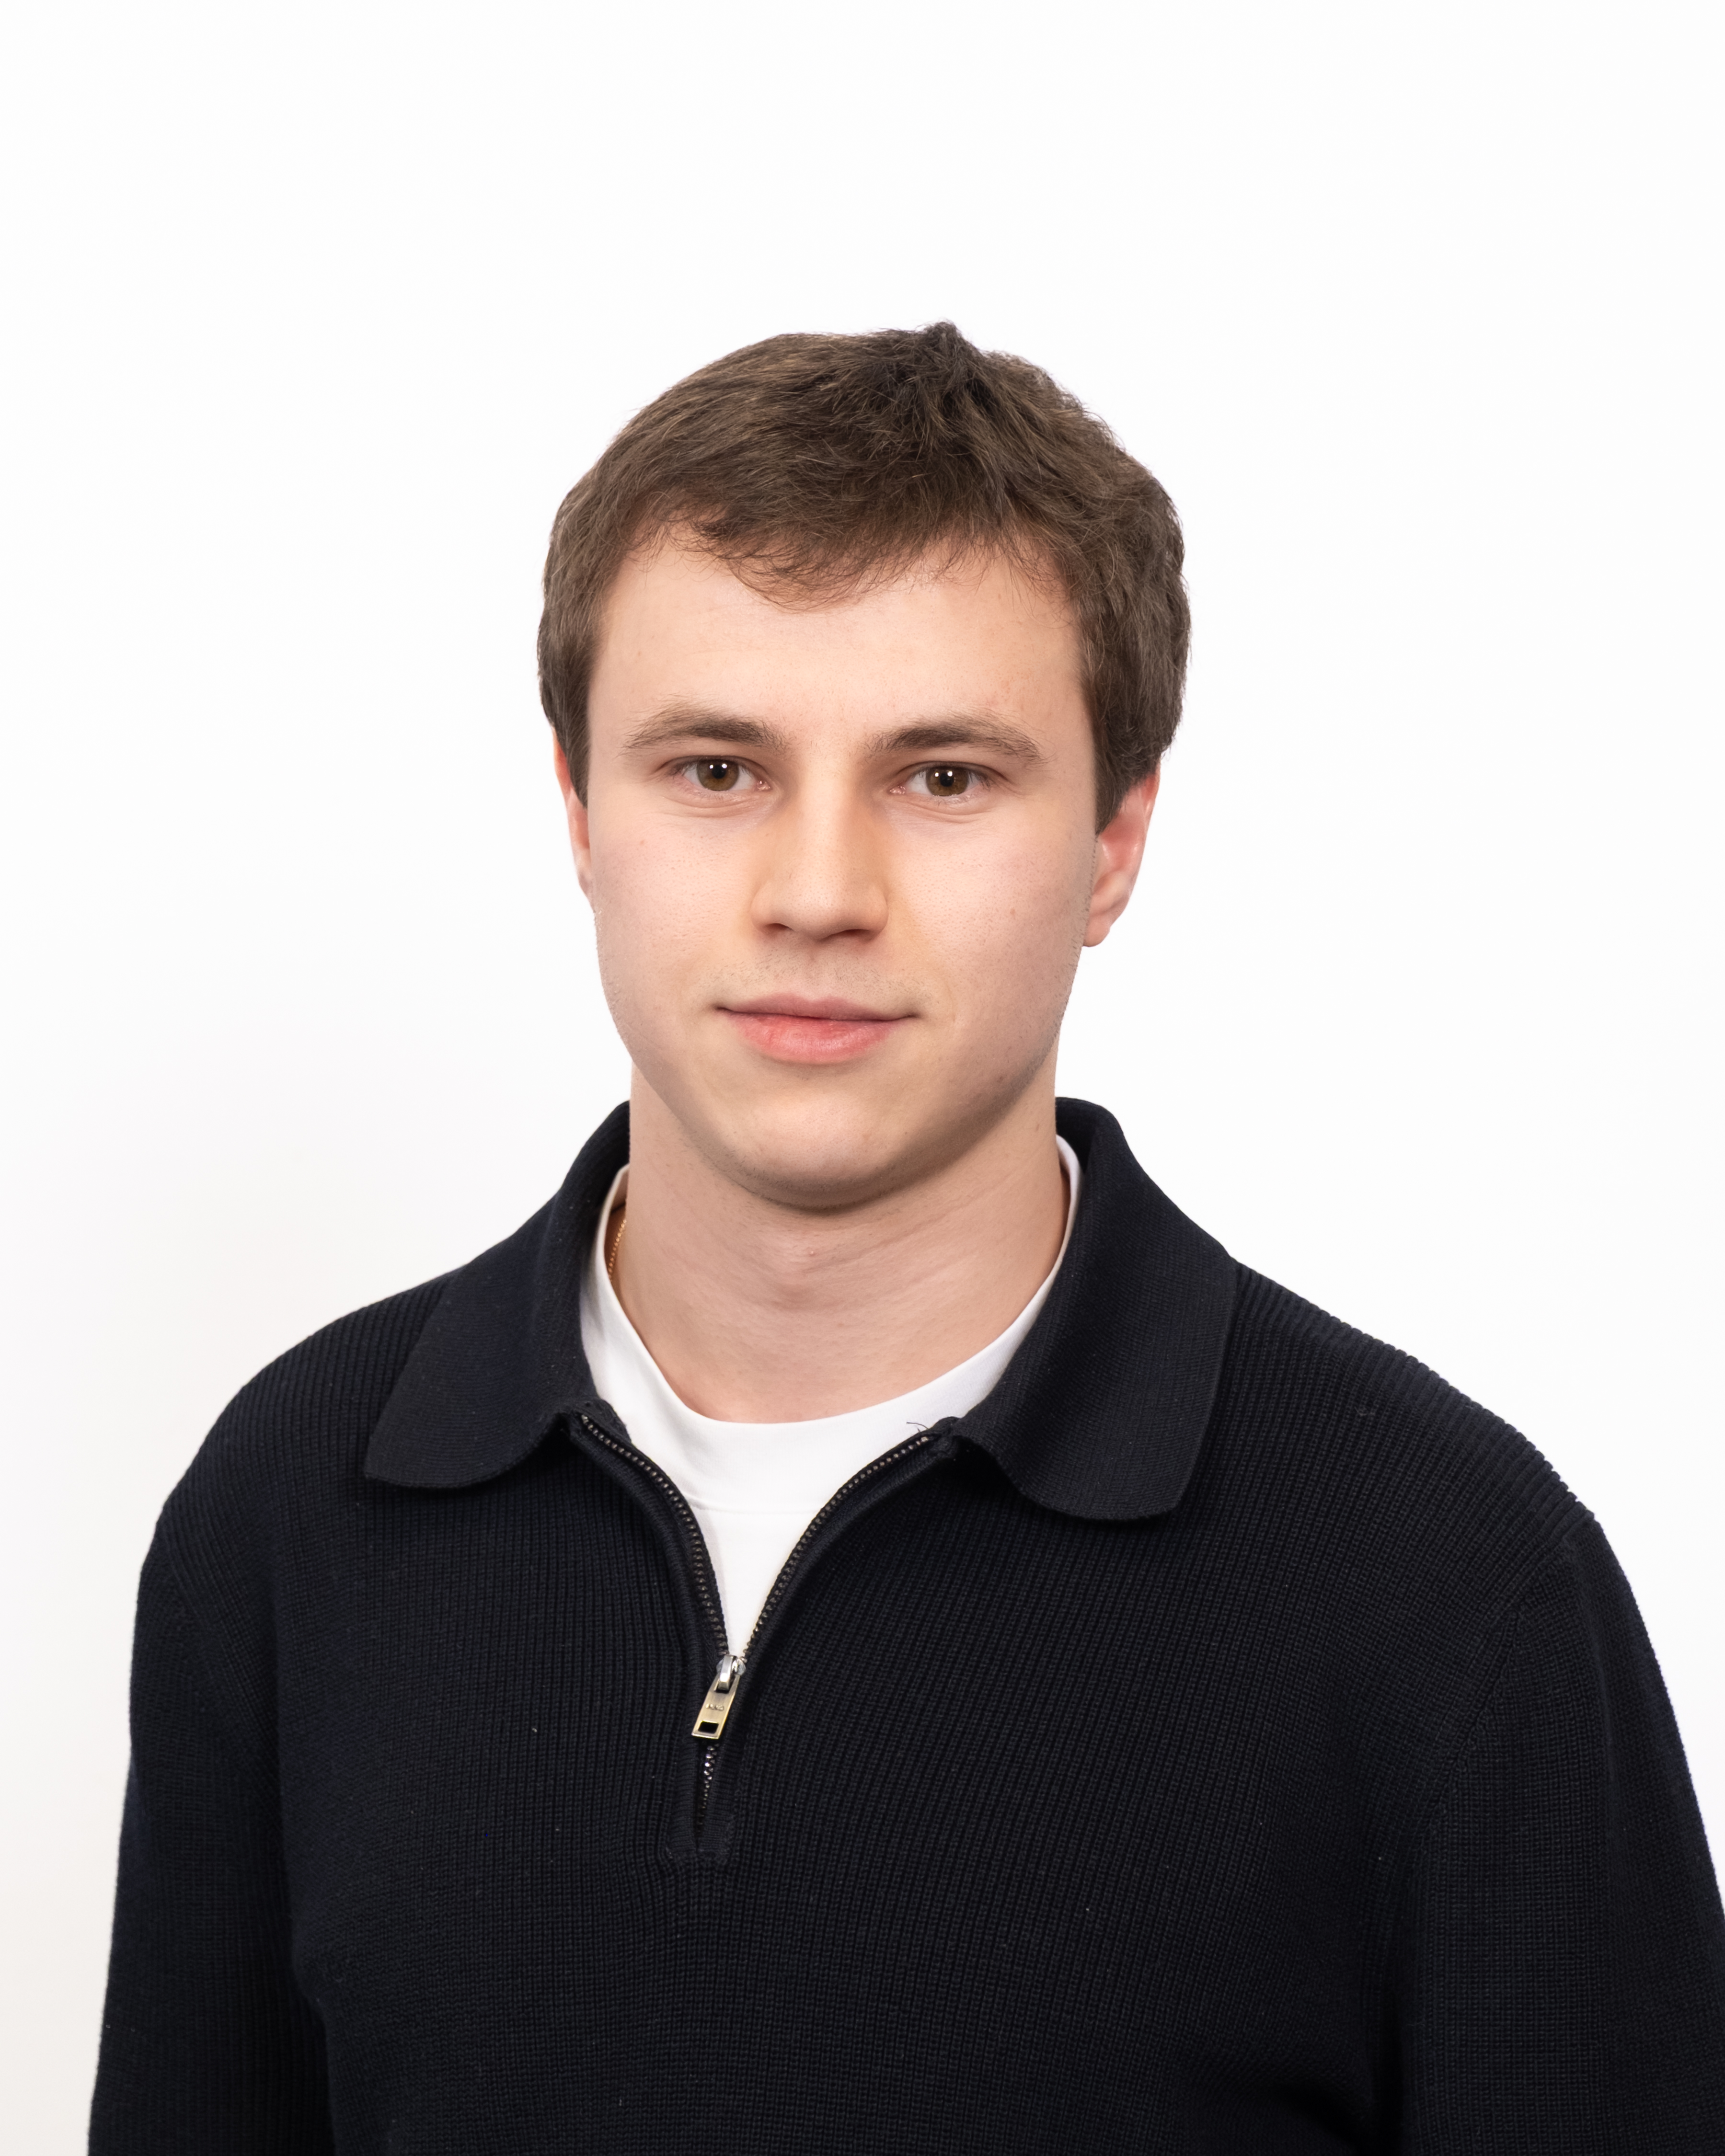
\includegraphics[width=1.6cm, keepaspectratio]{img/photo.png}};
    \end{tikzpicture}
\end{minipage}

%----------------------------------------------------------------------------------------
% PROFESSIONAL EXPERIENCE
%----------------------------------------------------------------------------------------
\vspace{-15pt}
\pdfbookmark[1]{Experience}{work_exp}
\cvsection{\workIcon[black]\hspace{4pt}PROFESSIONAL EXPERIENCE}

\vspace{-4pt}
\pdfbookmark[2]{Société Générale}{sg}
\cvevent{Data Engineer / MLOps (Work-study) --- Société Générale Assurances}{\fontsize{11pt}{11pt}\selectfont 09/2023\hspace{5pt}--\hspace{5pt}Present}
\cvsubevent{La Défense, France}{}

\vspace{-3pt}
\begin{itemize}[leftmargin=0.5cm, label=\textbullet, itemsep=0.0625em]
    \item Designed an \textbf{automated SAS-to-Python migration system} powered
          by \textbf{GitHub Copilot}, leveraging \textbf{prompt engineering},
          reusable \textbf{Skills} (specialized agent capabilities) and persistent
          context (\texttt{copilot-instructions.md}), validated by a 2-tier test suite
          \begin{itemize}[leftmargin=0.25cm,label=\textendash,itemsep=0em,topsep=0.2em]
              \item \textit{\fontsize{10pt}{9pt}\selectfont Python · Polars · DuckDB · GitHub Copilot · Prompt Engineering · AWS S3}
          \end{itemize}

    \item Data analysis on recognition errors of the \textbf{Zaion Callbot} based on
          \textbf{1 year of operational data} to evaluate \textbf{system effectiveness}
          and identify the main causes of errors, leading to \textbf{3 improvement
              recommendations}
          \begin{itemize}[leftmargin=0.25cm,label=\textendash,itemsep=0em,topsep=0.2em]
              \item \textit{\fontsize{10pt}{9pt}\selectfont Python · Pandas · NumPy · Matplotlib · Seaborn · Plotly · Jupyter Notebook · Conda}
          \end{itemize}

    \item Development and deployment of \textbf{3 VS-Code extensions} to simplify the use
          of internal tools on the \textbf{Data platform} and improve workflow efficiency
          for \textbf{30\raisebox{0.20ex}{\small +} users (Data Scientists \& Data
              Analysts)}
          \begin{itemize}[leftmargin=0.25cm,label=\textendash,itemsep=0em,topsep=0.2em]
              \item \textit{\fontsize{10pt}{9pt}\selectfont TypeScript · Python · JSON · Bash · Linux · Git · VS-Code}
          \end{itemize}

    \item Design and deployment of a \textbf{Zaion Callbot monitoring dashboard} to track
          \textbf{10\raisebox{0.20ex}{\small +} operational KPIs} and analyze system
          performance for internal teams
          \begin{itemize}[leftmargin=0.25cm,label=\textendash,itemsep=0em,topsep=0.2em]
              \item \textit{\fontsize{10pt}{9pt}\selectfont Apache Superset · PostgreSQL}
          \end{itemize}

    \item Design and automation of a \textbf{data migration pipeline} enabling the
          transfer of \textbf{500\raisebox{0.20ex}{\small +} GB of SAS datasets to AWS
              S3}, in order to improve \textbf{scalability, access, and data processing} for
          Data teams
          \begin{itemize}[leftmargin=0.25cm,label=\textendash,itemsep=0em,topsep=0.2em]
              \item \textit{\fontsize{10pt}{9pt}\selectfont Python · AWS S3 · fsspec · smbfs · Linux · Bash}
          \end{itemize}

          % \item Improvement of an \textbf{internal access management tool} to simplify the
          %       administration of \textbf{user rights} for \textbf{30\raisebox{0.20ex}{\small
          %               +} users} in Data teams
          %       \begin{itemize}[leftmargin=0.25cm,label=\textendash,itemsep=0em,topsep=0.2em]
          %           \item \textit{\fontsize{10pt}{9pt}\selectfont Python · JavaScript · API · Git}
          %       \end{itemize}

    \item Maintenance and update of \textbf{35\raisebox{0.20ex}{\small +} internal
              extensions} as well as \textbf{code-server versions} to ensure the
          \textbf{stability and compatibility of the development environment} used by
          \textbf{40\raisebox{0.20ex}{\small +} users} in Data teams
          \begin{itemize}[leftmargin=0.25cm,label=\textendash,itemsep=0em,topsep=0.2em]
              \item \textit{\fontsize{10pt}{9pt}\selectfont Linux · Bash · VS Code · code-server · Git}
          \end{itemize}

          % \item Analysis and comparison of \textbf{two data tables (SAS vs DataLake S3)} on
          %       \textbf{several thousand rows} via \textbf{matching methods and gap analysis},
          %       enabling the identification of \textbf{data inconsistencies and discrepancies}
          %       in a migration project
          %       \begin{itemize}[leftmargin=0.25cm,label=\textendash,itemsep=0em,topsep=0.2em]
          %           \item \textit{\fontsize{10pt}{9pt}\selectfont Python · Pandas · SAS · AWS S3 · Jupyter Notebook · Git}
          %       \end{itemize}
\end{itemize}

% \pdfbookmark[2]{IT Company SPD}{spd}
% \vspace{-5pt}
% \cvevent{\textbf{Training at IT Company SPD Ukraine} --- Machine Learning / Deep Learning}{\fontsize{11pt}{11pt}\selectfont 2022}
% \cvsubevent{}{Cherkasy, Ukraine}
% \vspace{-18pt}
% \begin{itemize}[leftmargin=0.75cm,label=\textendash,itemsep=0em,topsep=0.2em]
%     \item \textit{\fontsize{10pt}{9pt}\selectfont Scikit-Learn · Pandas · NumPy · Matplotlib · Seaborn · TensorFlow · XGBoost}
% \end{itemize}

%----------------------------------------------------------------------------------------
% IT PROJECTS
%----------------------------------------------------------------------------------------
\vspace{-5pt}
\pdfbookmark[1]{Projects}{projects}
\vspace{-1pt}
\cvsection{\itProjectIcon[black]\hspace{4pt}IT PROJECTS}

\vspace{-4pt}
\begin{itemize}[leftmargin=0.5cm, label=\textbullet, itemsep=0.2em]
    \pdfbookmark[2]{Phishing email detection}{phishing}
    \item \href{https://github.com/DmytroPalahin/phishing-email-detection}{\textbf{Phishing Email Detection System}} | \textit{Python, Machine Learning, NLP} \hfill \textbf{2026}

          Phishing email classifier trained on \textbf{76\,677 emails} (5 real-world datasets) via
          full NLP pipeline~: TF-IDF, URL extraction, LightGBM\,+\,Naive Bayes\,+\,LSTM ensemble
          %   \begin{itemize}[leftmargin=0.25cm,label=\textendash,itemsep=0em,topsep=0.2em]
          %       \item \textit{\fontsize{10pt}{9pt}\selectfont Python · LightGBM · TensorFlow/Keras · Scikit-Learn · Pandas · NumPy · Jupyter}
          %   \end{itemize}

          \pdfbookmark[2]{Logistics Center Placement}{logistics}
    \item \href{https://github.com/DmytroPalahin/logistics-center-placement}{\textbf{Logistics Center Placement}} | \textit{Python, Julia, CPLEX, Optimization} \hfill \textbf{2025}

          Combinatorial optimization project for logistics center placement using MILP
          models solved with CPLEX and heuristics

          \pdfbookmark[2]{Reaction System}{rs}
    \item \href{https://github.com/DmytroPalahin/hsReact}{\textbf{Reaction System}} | \textit{Haskell} \hfill \textbf{2024}

          Representation of reaction systems and processes using functional programming

          \pdfbookmark[2]{Traveling Salesman Problem}{salesman}
    \item \href{https://github.com/DmytroPalahin/Probleme_du_Voyageur_de_Commerce}{\textbf{Traveling Salesman Problem}} | \textit{C, Reinforcement Learning} \hfill \textbf{2023}

          Implementation of the ant colony optimization algorithm

          \pdfbookmark[2]{Article}{article}
    \item \href{https://www.researchsquare.com/article/rs-2203260/v1}{\textbf{Research Publication}} | \textit{Mathematical Algorithms} --- Impulse noise filtering method in video images \textit{Informatics and Mathematical Methods in Simulation}, Vol. 11 (2021), No. 4 \hfill \textbf{2021}

          \pdfbookmark[2]{Anomaly Detection}{anomaly_detection}
    \item \href{https://github.com/DmytroPalahin/Anomaly_Detection}{\textbf{Anomaly Detection}} | \textit{Python, Machine Learning} \hfill \textbf{2021}

          Methods for partial data labeling

          %       \pdfbookmark[2]{Image Filtering}{filtering_imgs}
          % \item \href{https://github.com/DmytroPalahin/Filtering_Images}{\textbf{Image Filtering}} | \textit{HTML, CSS, JS, Algorithms} \hfill \textbf{2019}

          %       Implementation of mathematical methods for noise filtering in digital images
          %       as a web service
\end{itemize}

%----------------------------------------------------------------------------------------
% EDUCATION
%----------------------------------------------------------------------------------------
\vspace{-5pt}
\pdfbookmark[1]{Education}{education}
\cvsection{\educationIcon[black]\hspace{4pt}EDUCATION}

\vspace{-3pt}
\pdfbookmark[2]{Sup Galilée}{sup_galilee}
\cvevent{\href{https://www.sup-galilee.univ-paris13.fr/}{Sup Galilée Engineering School} --- Engineering Degree in Computer Science}{\fontsize{11pt}{11pt}\selectfont 2023\hspace{5pt}--\hspace{5pt}2026}
% \cvsubevent{}{Villetaneuse, France}

\vspace{-3pt}
\cvtextnotab{\textbf{Courses\!:} Cloud Computing, Data Mining and Programming for AI, Databases (MySQL) and NoSQL, Docker, Probability and Statistics, Linear and Combinatorial Optimization, Parallel and Distributed Algorithms, Graph Algorithms, and others}
% additional courses:
% Cybersecurity
% UML
% Analysis / Algebra
% Cryptography
% Complexity
% Compilation and language theory
% Functional programming
% Logic programming
% System administration
% Network administration
% Computer architecture
% Numerical methods
% Semantic web
% Logic
% Operating systems
% C/C++
% Web (TS/JS)

\vspace{-10pt}
\noindent{\textcolor{middle_light_gray}{\rule{\mpwidth}{0.2pt}}}
\vspace{-15pt}

\pdfbookmark[2]{Preparatory Class}{prepa}
\cvevent{\href{https://www.univ-spn.fr}{Sorbonne Paris Nord University} --- \href{https://www.sup-galilee.univ-paris13.fr/index.php/formation/cp2i/}{Preparatory Class for \textbf{Sup Galilée}}}{\fontsize{11pt}{11pt}\selectfont 2021\hspace{5pt}--\hspace{5pt}2023}
% \cvsubevent{}{Villetaneuse, France}

\vspace{-10pt}
\cvtextnotab{\textbf{Courses\!:} Algebra, Analysis, Topology and Differential Calculus, Scientific Computing, Algorithms, UNIX Systems}

% \vspace{-5pt}
% \noindent{\textcolor{middle_light_gray}{\rule{\mpwidth}{0.2pt}}}
% \vspace{-10pt}

% \pdfbookmark[2]{High School}{high_school}
% \cvevent{Phymly High School --- Specialization in Mathematics, Physics and Computer Science}{\fontsize{11pt}{11pt}\selectfont 2016\hspace{5pt}--\hspace{5pt}2021}
% \cvsubevent{}{Cherkasy, Ukraine}

%----------------------------------------------------------------------------------------
% CERTIFICATIONS & SKILLS
%----------------------------------------------------------------------------------------
\vspace{-14pt}
\pdfbookmark[1]{Certifications and Skills}{certifications_competences}
\cvsection{\certificateIcon[black]\hspace{4pt}CERTIFICATIONS \& SKILLS}

\vspace{-4pt}
\begin{itemize}[leftmargin=0.5cm, label=\textbullet, itemsep=0.2em]
    \item \textbf{Languages \& Tools\!:}
          Python, SQL, JS/TS, Java, C/C++, Haskell, Julia, Matlab, LaTeX ·
          Pandas, NumPy, Polars, Scikit-Learn, TensorFlow, Keras, LightGBM, XGBoost ·
          Matplotlib, Seaborn, Plotly ·
          Apache Spark, PySpark ·
          Jupyter, Anaconda, UV, Docker, Git, Wireshark, Jira ·
          Linux, Windows, macOS

    \item \textbf{Udemy --- Jose Portilla / Pierian Training\!:}
          \href{https://www.udemy.com/certificate/UC-51319000-ccb8-4c9c-9320-6cd9860e601c/}
          {\textit{Python for Data Science and Machine Learning Bootcamp}}
          |
          \textit{Python, NumPy, Pandas, Scikit-Learn, Matplotlib, Seaborn, Plotly,
              Machine Learning, NLP, Deep Learning, TensorFlow/Keras, Apache Spark}

    \item \textbf{Huawei AI Certifications:}
          \href{https://github.com/DmytroPalahin/cv-latex-simple-en/blob/main/docs/huawei_artificial_intelligence_and_applications.pdf}
          {\textit{Artificial Intelligence and Applications}}
          \hspace{4pt}•\hspace{4pt}
          \href{https://github.com/DmytroPalahin/cv-latex-simple-en/blob/main/docs/huawei_artificial_intelligence_technology_and_applications.pdf}
          {\textit{Artificial Intelligence Technology and Applications}}

          % \item \textbf{SPD Ukraine\!:} Training in Machine Learning in an IT company
          % \item \textbf{Stepik\!:} Training in Machine Learning
\end{itemize}

%----------------------------------------------------------------------------------------
% AWARDS & PARTICIPATIONS
%----------------------------------------------------------------------------------------
\vspace{-3pt}
\pdfbookmark[1]{Participations}{participations}
\cvsection{\awardIcon[black]\hspace{4pt}AWARDS \& PARTICIPATIONS}

\vspace{-6pt}
\begin{itemize}[leftmargin=0.35cm, label=\textbullet, itemsep=0.15em]
    \item \textbf{\href{https://www.fondationbesse.com/}{Georges Besse Foundation Laureate}}
    \item \textbf{Eco\hspace{3pt}--\hspace{3pt}Techno Ukraine ISEF} --- 1\textsuperscript{st} place in Computer Science \& \textbf{Collective Intelligence Internet Service} --- 1\textsuperscript{st} place in Ukraine
\end{itemize}

%----------------------------------------------------------------------------------------
% LANGUAGES & INTERESTS
%----------------------------------------------------------------------------------------
\vspace{-5pt}
\pdfbookmark[1]{Languages and interests}{languages_interests}
\cvsection{\speechBubbleIcon[black]\hspace{4pt}LANGUAGES \& INTERESTS}

\vspace{-3pt}
\cvtextnotab{\textbf{English\!:} Fluent \hspace{12pt} \textbf{French\!:} Fluent \hspace{12pt} \textbf{Ukrainian\!:} Native \hspace{20pt} \textbf{Russian\!:} Bilingual}

\vspace{-8pt}
\cvtextnotab{
    \tradingIcon[black]\hspace{2pt}Investing \hspace{12pt}
    % \cryptoIcon[black]\hspace{2pt}Crypto \hspace{12pt}
    \chessIcon[black]\hspace{2pt}Chess \hspace{12pt}
    \skiIcon[black]\hspace{2pt}Skiing \hspace{12pt}
    \tennisIcon[black]\hspace{2pt}Tennis \hspace{12pt}
    \swimmingIcon[black]\hspace{2pt}Swimming \hspace{12pt}
    % \mountainsIcon[black]\hspace{2pt}Hiking
    \flagIcon[black]\hspace{2pt}Karting | Formula 1
}

\end{document}

/*
latexmk -pdf cv-dmytro-palahin-en-d.tex
latexmk -pdf -auxdir=/tmp/latex-build -outdir=. cv-dmytro-palahin-en-d.tex
pdftoppm -png -r 600 cv-dmytro-palahin-en-d.pdf ./img/cv-dmytro-palahin-en-d
*/
